\section{Case study}
\label{case}
In Belgium, when a party wants to conclude a transaction on the real estate
market, a notary is required to affirm the process, providing legal certificates for the requested transaction. 
This registration gives rise to the payment of registration duties, which depend on the region in which the estate is situated. 
The standard tax rate can be reduced for certain registration types, which leads to a range of possible tax rates with their associated conditions.\footnote{For the Flemish region the applicable legislation is the "Decreet van 13 december 2013 houdende de Vlaamse codex fiscaliteit" with amending decrees from December 19th 2014 and May 18th 2018.}

Prior to June 1st 2018, the central concept to determine the registration type was the \textit{kadastral income (KI)}, a value which represents its theoretical rental value. 
%Only for some houses this value got reviewed to current standards. 
%This KI was then compared to a threshold, that depended on the buyer's number of children.
In the new legislation, the concept of \textit{KI} was abandoned. 
To determine if a house should be considered ``modest'',  its actual selling price is now used instead of the fictitious \textit{KI}.
%For such modest houses, a fixed discount replaces the\textit{ abattement}.
The reforms of the registration duties represent a profound change: of the original 42 articles of chapter 9 concerning the registration law, the decree of May 18th 2018 abolishes 4 articles, modifies 9 and adds 5.% \cite{newlaw}.
\begin{comment}
Our prototype of \cite{ruleml/DeryckHVV18} employs a knowledge base for the original legislation. Its functionality focuses on two requirements:
\begin{compactitem}
\item \emph{Completeness and correctness:} The application should ensure that all possible discounts are taken into account, and only rule out or apply discounts when warranted by the information provided by the notary. 

\item \emph{Usability:}  In meetings between notaries and their clients, the technology should not disturb the confidential atmosphere.  A lot of typing and searching for the correct button is out of the question. 
\end{compactitem}

After evaluating this prototype, the notary office came up with these additional requirements:
\begin{compactitem}
\item \emph{Traceability}  The decision outcomes calculated by the application should be easy to check and explain,  in order to increase clients' confidence in the application.  
\item \emph{Efficient information gathering}  Only questions relevant to possible discounts should be asked. E.g., as soon as it is clear that one of the discounts cannot be used, questions related to this discount become irrelevant and should no longer be asked.
\end{compactitem}

\section{Original prototype}
\label{original}

\begin{figure*}[]
	\centering	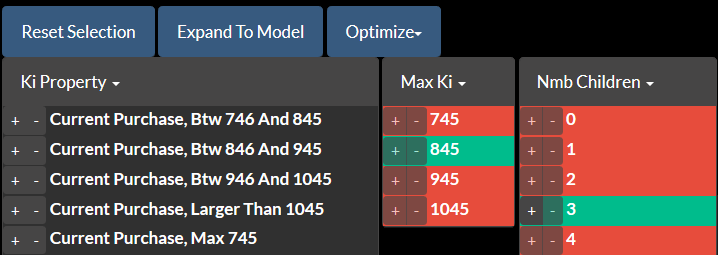
\includegraphics[angle=0,width = 0.6\linewidth]{img/oldscreen_joost.png} %, trim={2.5cm 21,7cm 2,2cm 2,0cm}, clip]
	\caption{Propagation in the original prototype.}
	\label{fig:old}
\end{figure*}
\end{comment}

At the start of the case study the notary's application requirements were rather vague.
The most important concern was to use the obtained information in an intelligent way, i.e., use the information instantly to derive conclusions.
Because of this we opted for the use of an earlier developed \textit{automatic configuration} interface available online \cite{idphome}.
%As the use of it is independent of the domain described in the vocabulary and theory in the knowledge base, this was an easy way to create a first visual prototype to solicit further application requirements from the notary\cite{ruleml/DeryckHVV18}.
In this prototype, the user is presented a list of unknown \emph{atomic} statements (e.g., whether the property can be considered ``modest'') which can be assigned appropriate truth values.
The prototype continuously \emph{propagates} all consequences following from such assignments under the rules specified by registration duty law, further restricting the values of the atoms.
In addition, the user may also request an \emph{expansion} of the current assignment to a satisfying configuration, which optionally minimizes the duties that need to be paid.

After evaluating this prototype, the notary office came up with two additional requirements.
First, \emph{traceability}: the outcomes propagated by the application should be easy to check and explain,  in order to increase clients' confidence in the application.  
Second, \emph{efficient information gathering}: only questions relevant to possible discounts should be asked. E.g., as soon as it is clear that one of the discounts cannot be used, atoms related to this discount become irrelevant and should no longer displayed.

\begin{comment}

As the former version of the legislation concerning registration duties  was unstructured and difficult to read, the model was built on more accessible information from the Federal Public Service Finance \cite{FODFinancien}. 
We analyzed and formalized the domain using the Decision Model and Notation (DMN) methodology.\footnote{The reasons and way of working with DMN are discussed in our earlier work, see \cite{ruleml/DeryckHVV18}.}
This resulted in a model consisting of a glossary and multiple connected decision tables. 
This was then translated into the IDP-language.
\end{comment}
The initial prototype formalizes 11 articles of law, resulting in a knowledge base of 53 concepts, 6 constraints and 14 rules \cite{ruleml/DeryckHVV18}. Building this knowledge base required an effort of approximately 10 person-days.
A significant part of this time was attributed to the creation of the set of symbols representing concepts in the domain, i.e. the \emph{vocabulary}. 

To evaluate the maintainability of the knowledge base, we examined the effort necessary to update it to the changes in legislation enacted in 2018. 
These changes consisted of 5 new articles, making it the most significant change to real estate sales law since the transfer of jurisdiction from the national to the Flemish regional government in 2013. 
At the time of constructing the original knowledge base, the content of these changes was not yet known.
Therefore, this provides a realistic test case to judge the maintainability of the knowledge base.

Updating the knowledge base required only $0.5$ person-days, a fraction of the time required for the initial version. 
16 of the original 53 concepts were removed and 18 new ones added; 11 existing constraints and rules needed to be updated or deleted, while 4 new constraints were added. 
Crucially, 9 of the 20 existing constraints/rules did not need to be touched at all. 
This demonstrates that the inherent modularity of the KBP indeed leads to significant advantages in practice.